\chapter{Etat de l'art}
\par
    % La première étape de mon stage consiste à créer un module de reconstruction 3D dans le framework SolAR. Ce module est très complexe et demanderait énormément de travail pour pouvoir être créer à partir de zéro. On va donc chercher un framework sous licence libre afin de pouvoir l'utiliser et/ou le modifier à volonté.

    % Afin de trouver le framework le plus adapté à notre utilisation, on va faire un état de l'art de tous les frameworks de reconstruction 3D. Il y a plusieurs critères important qui nous permettront de faire notre choix. On va en priorité regarder la licence des frameworks pour les raisons evoquées plus tôt. Ensuite comme SolAR est codé en C++ on cherche un framework principalement écrit dans le même langage. Enfin l'efficacité du framework est aussi un des critères recherchés durant cet état de l'art. Ici l'efficacité comprend la qualité du modèle 3D obtenu et la vitesse d'exécution.

Introduction / Pourquoi on fait cette étape

\section{Préparatifs}

Présentation des datasets utilisés (nb images, taille image, insideout/outside in)

\begin{figure}[ht]
    \centering
    \begin{subfigure}{0.40\textwidth}
        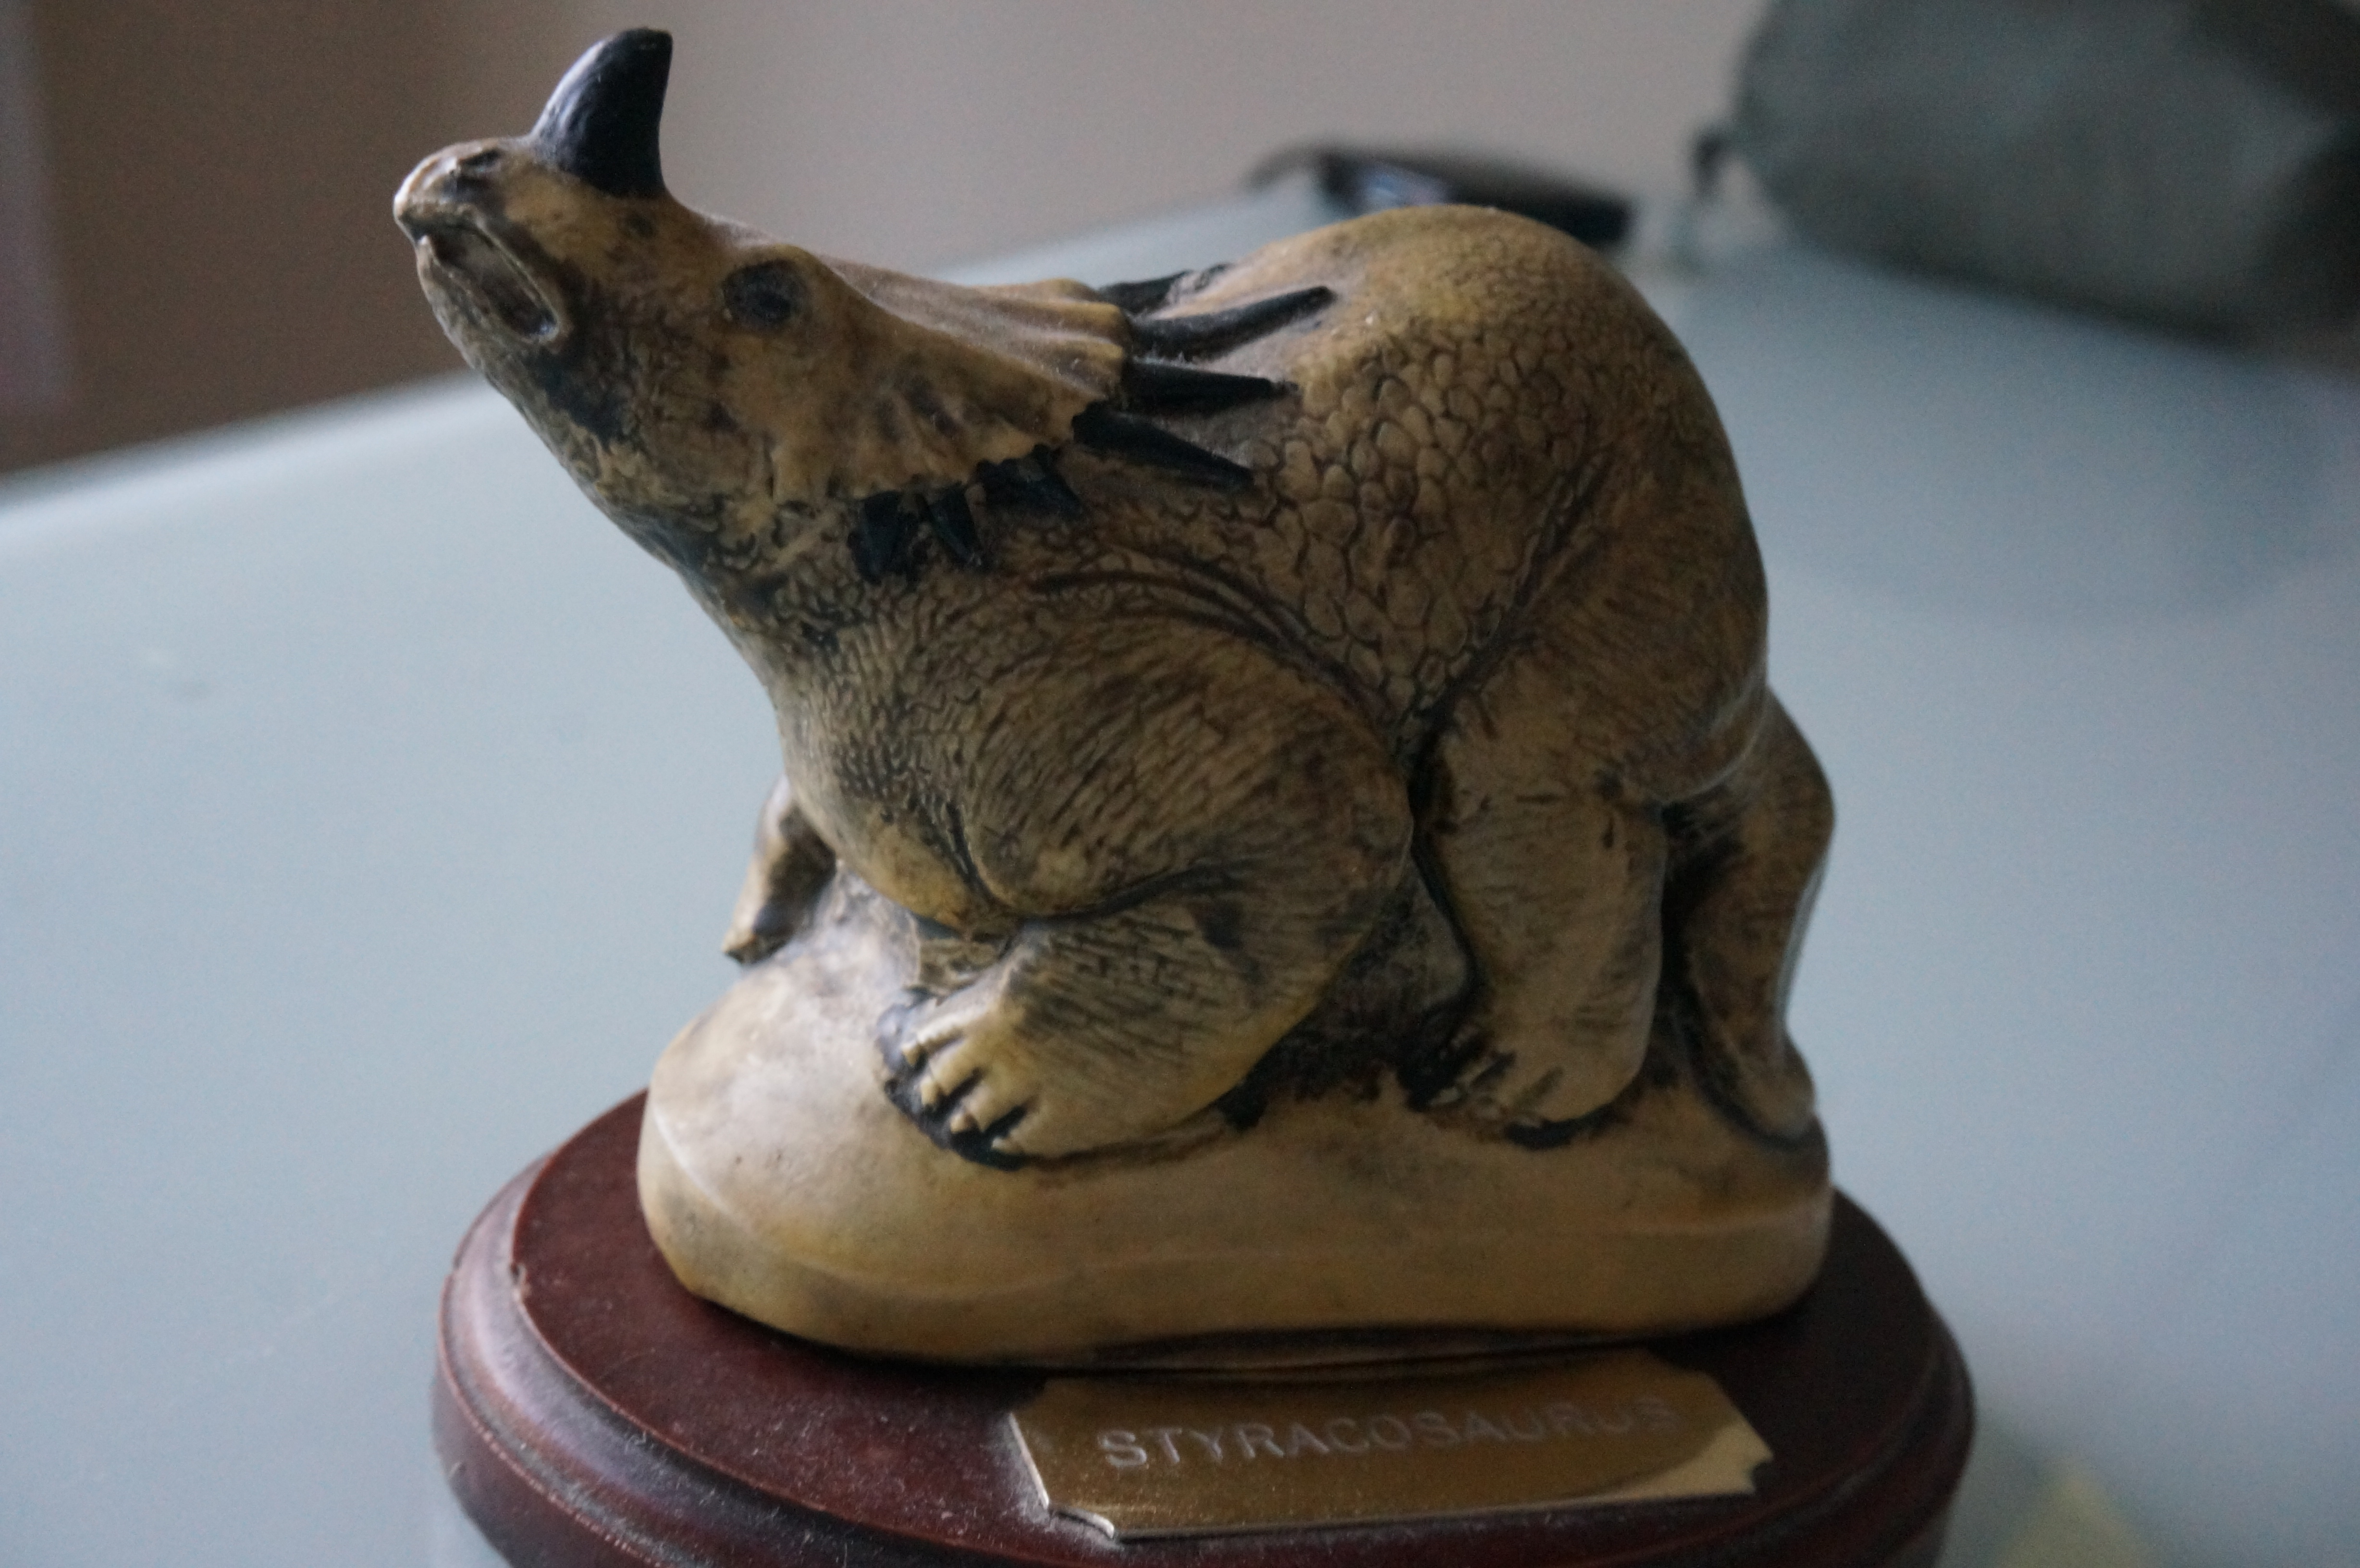
\includegraphics[width=\linewidth]{datas/dino_image.jpg}
        \caption{}
    \end{subfigure}
    \begin{subfigure}{0.47\textwidth}
        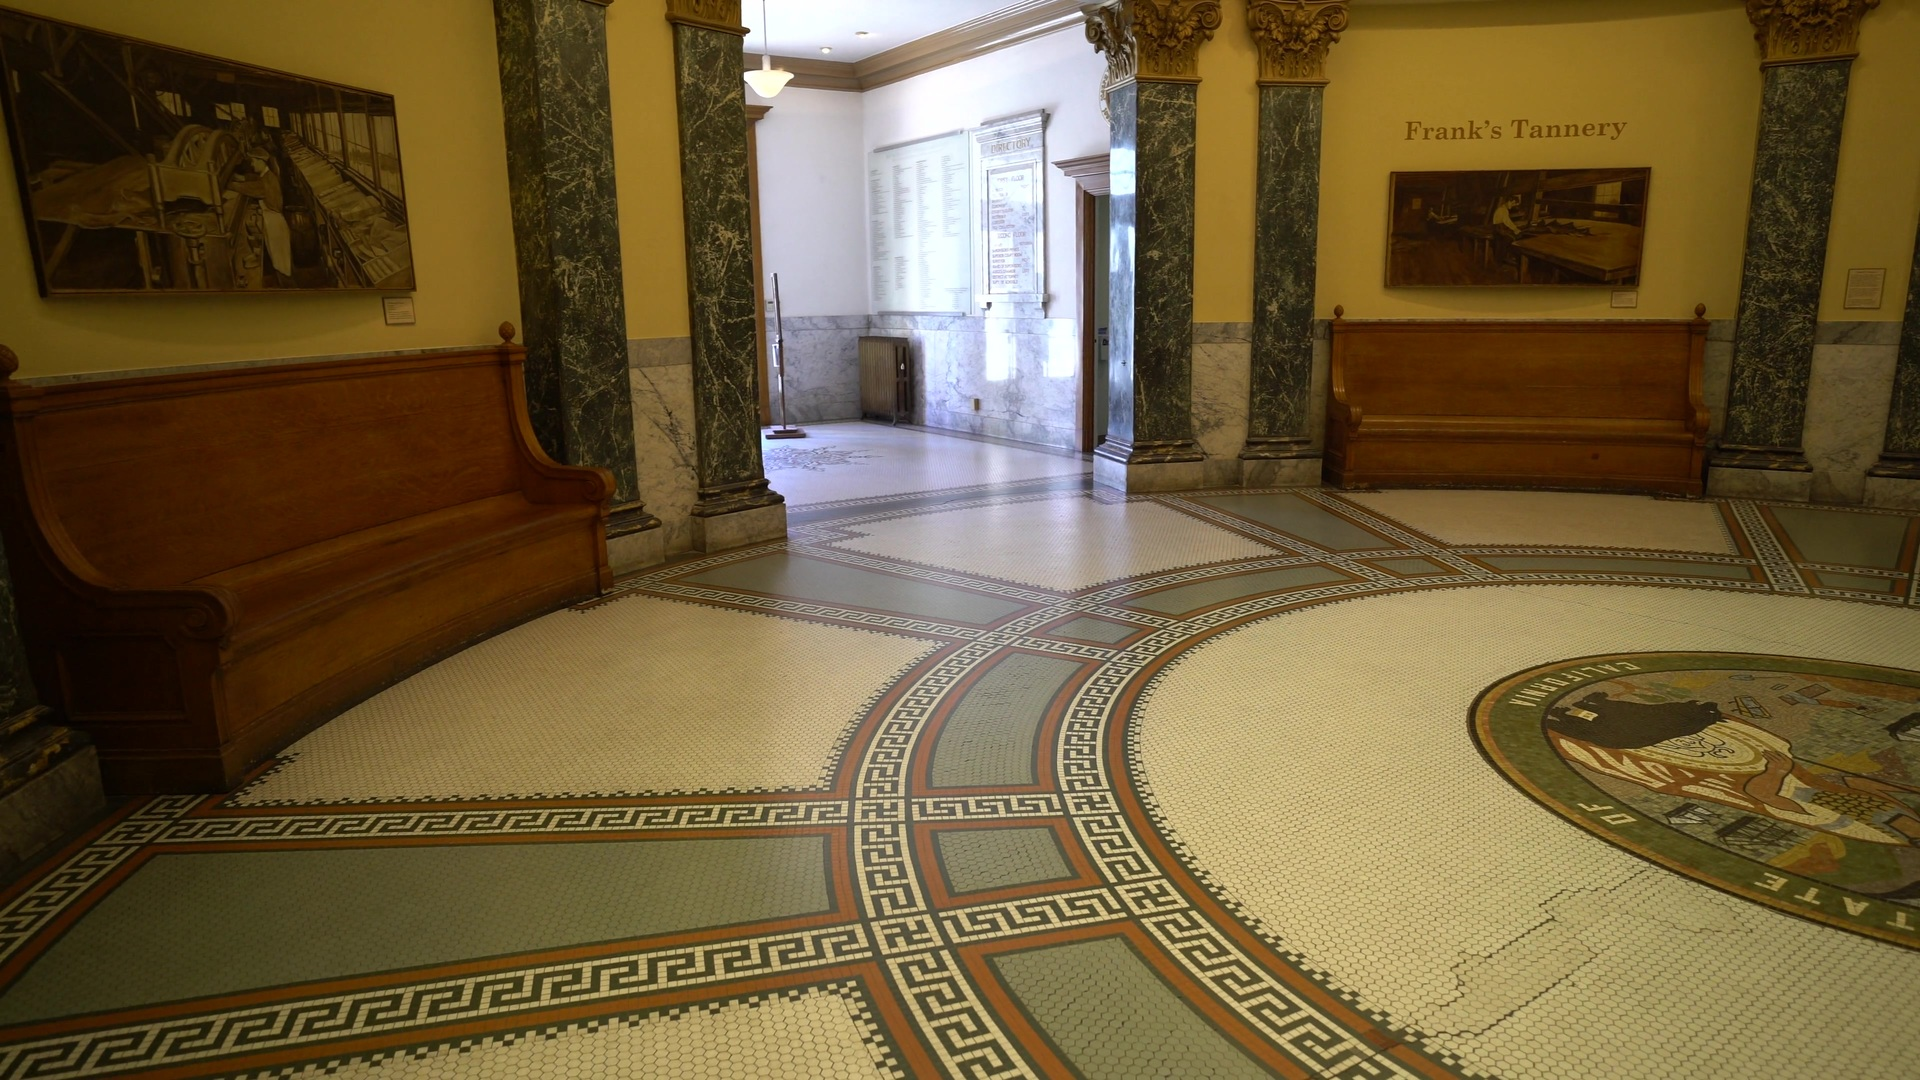
\includegraphics[width=\linewidth]{datas/museum_image.jpg}
        \caption{}
    \end{subfigure}

    \caption{Extrait du dataset \emph{Dinosaure} (a) et du dataset \emph{Museum} (b)}
    \label{fig:dataset_exemple}
\end{figure}

Explication des différents critères recherchés (C++, libre de droits, ...)

\section{Présentation des logiciels}

Présentation des différents softwares
\begin{itemize}
    \item OpenSFM
    \item VisualSFM
    \item OpenMVG + OpenMVS
    \item Alicevision Meshroom
    \item Regard3D
    \item Colmap
\end{itemize}

Affichage des résultats

\comment{Placé ici temporairement, surement déplacé en annexe après}

\begin{figure}[ht]
    \centering
    \begin{subfigure}{0.45\textwidth}
        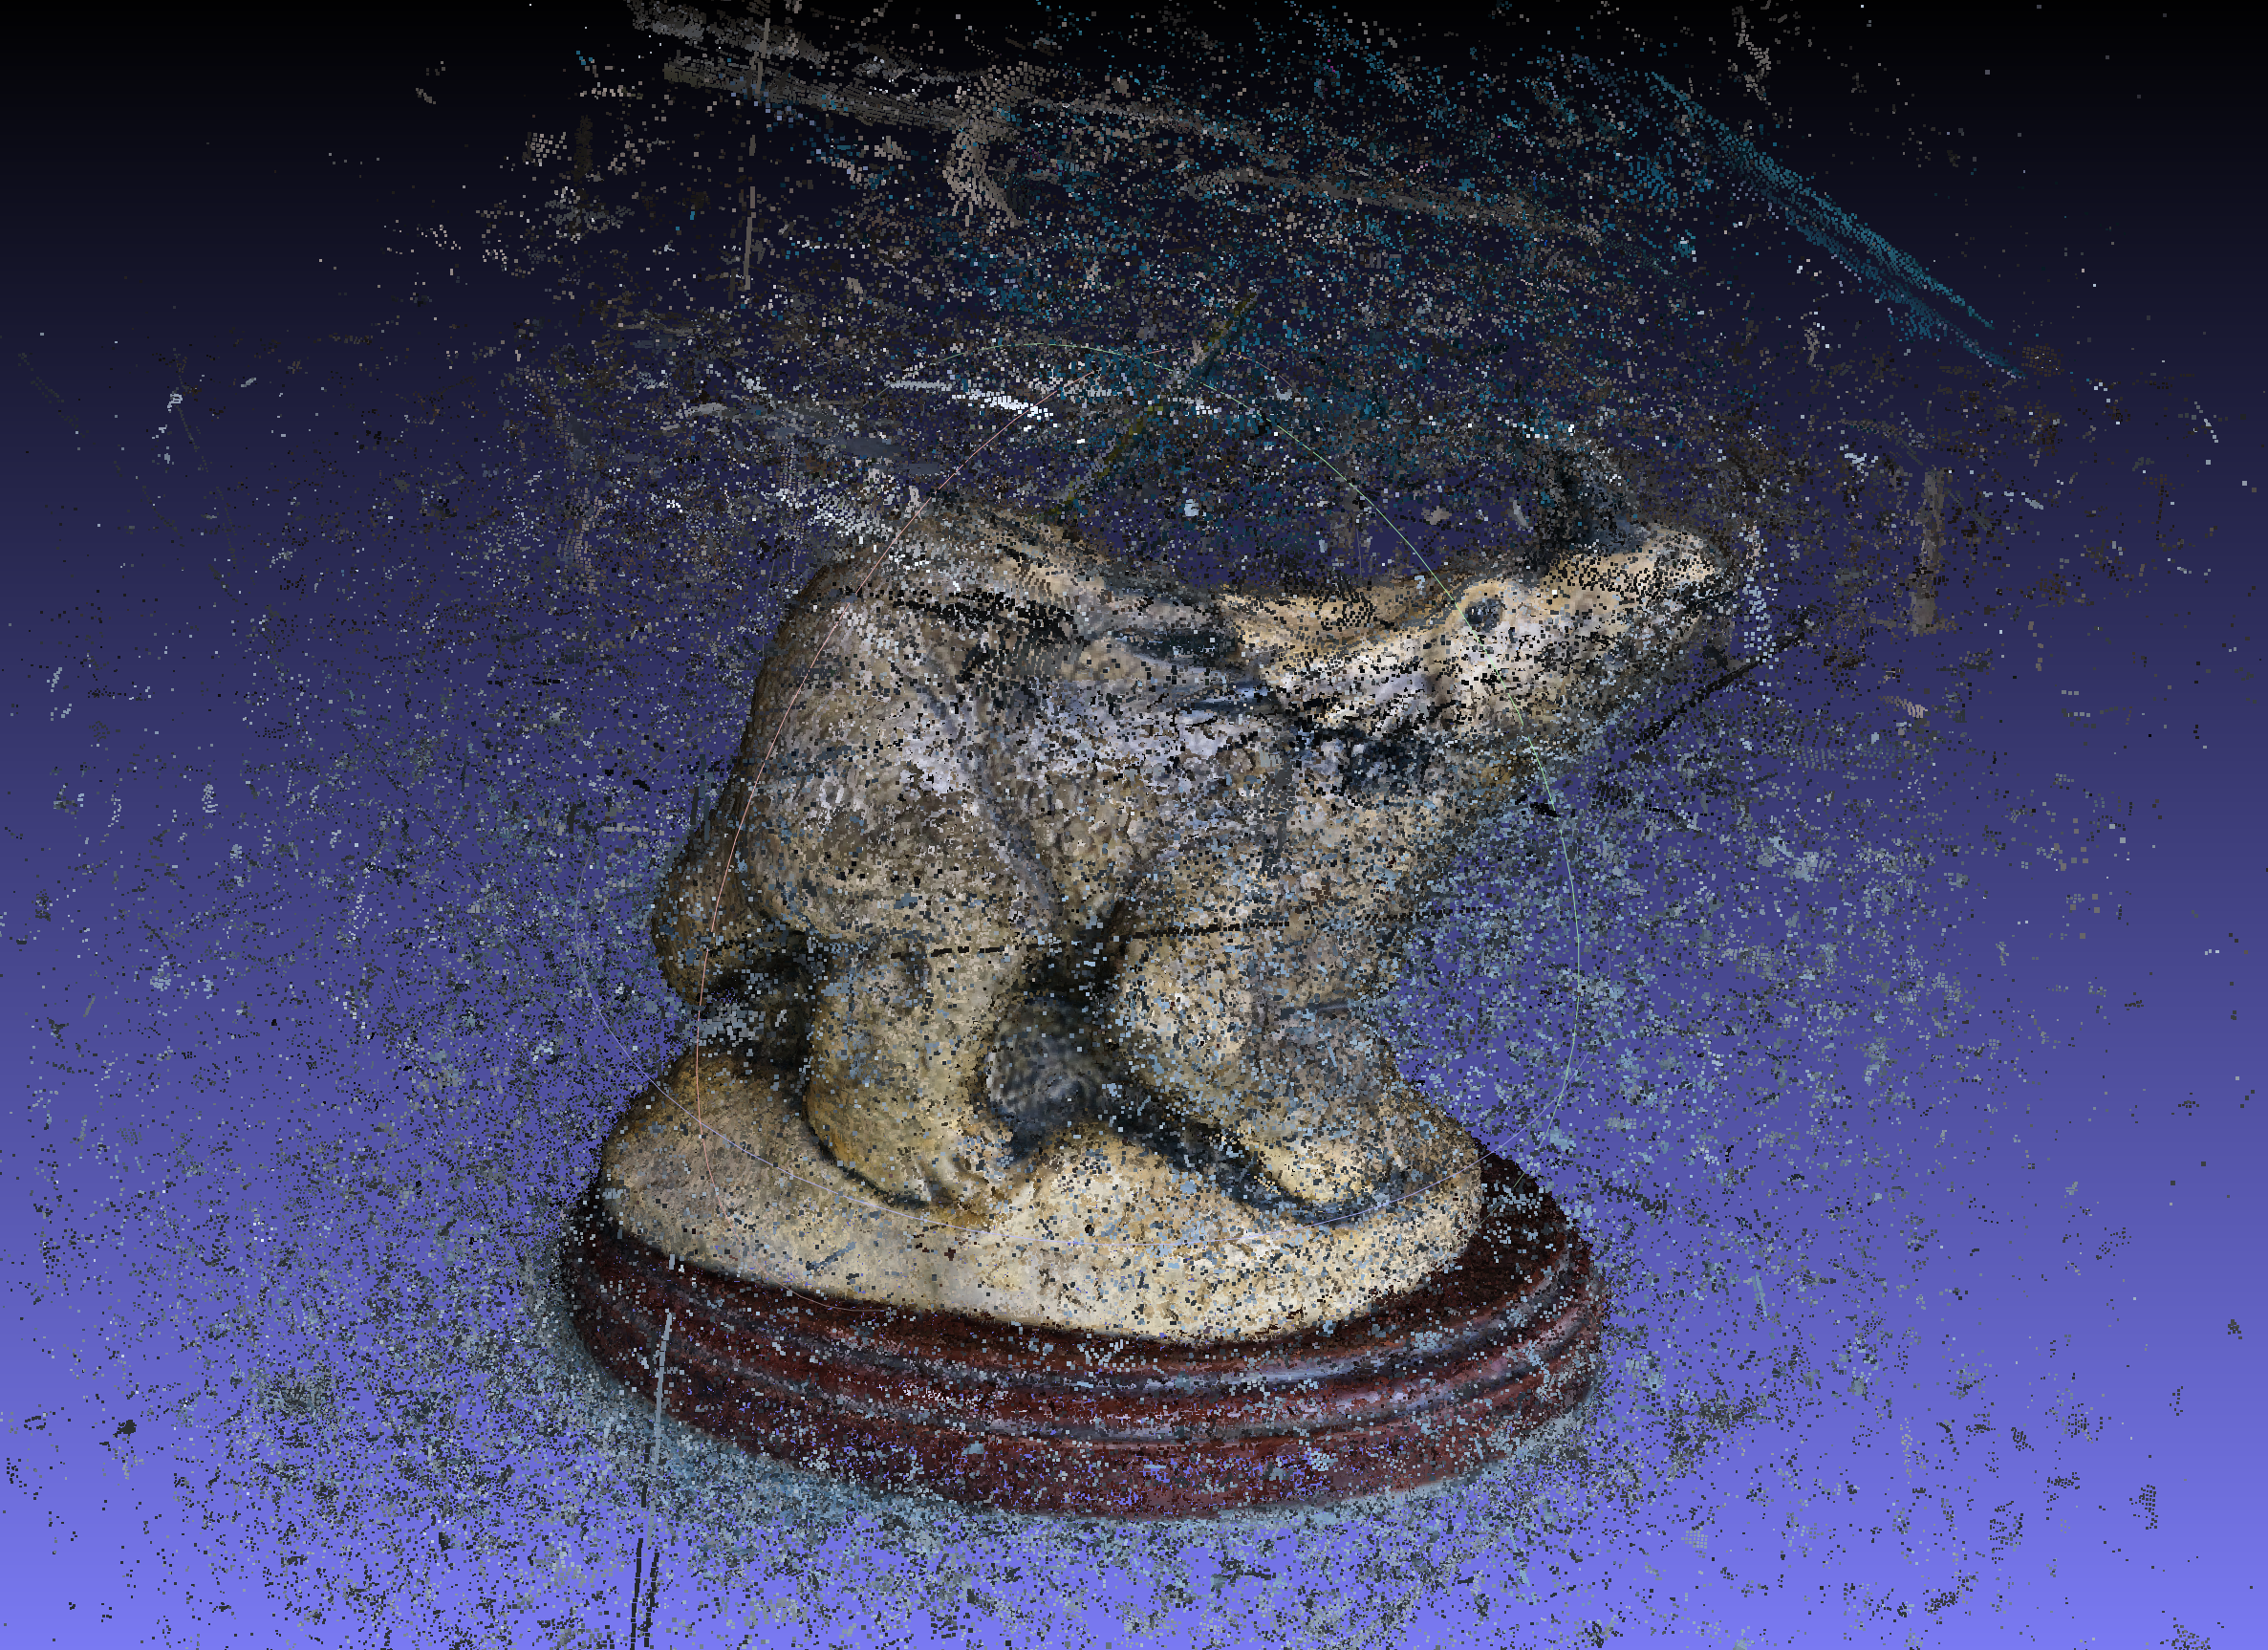
\includegraphics[width=\linewidth]{datas/state_of_the_art/opensfm_result_dino.png}
        \caption{}
    \end{subfigure}
    \begin{subfigure}{0.45\textwidth}
        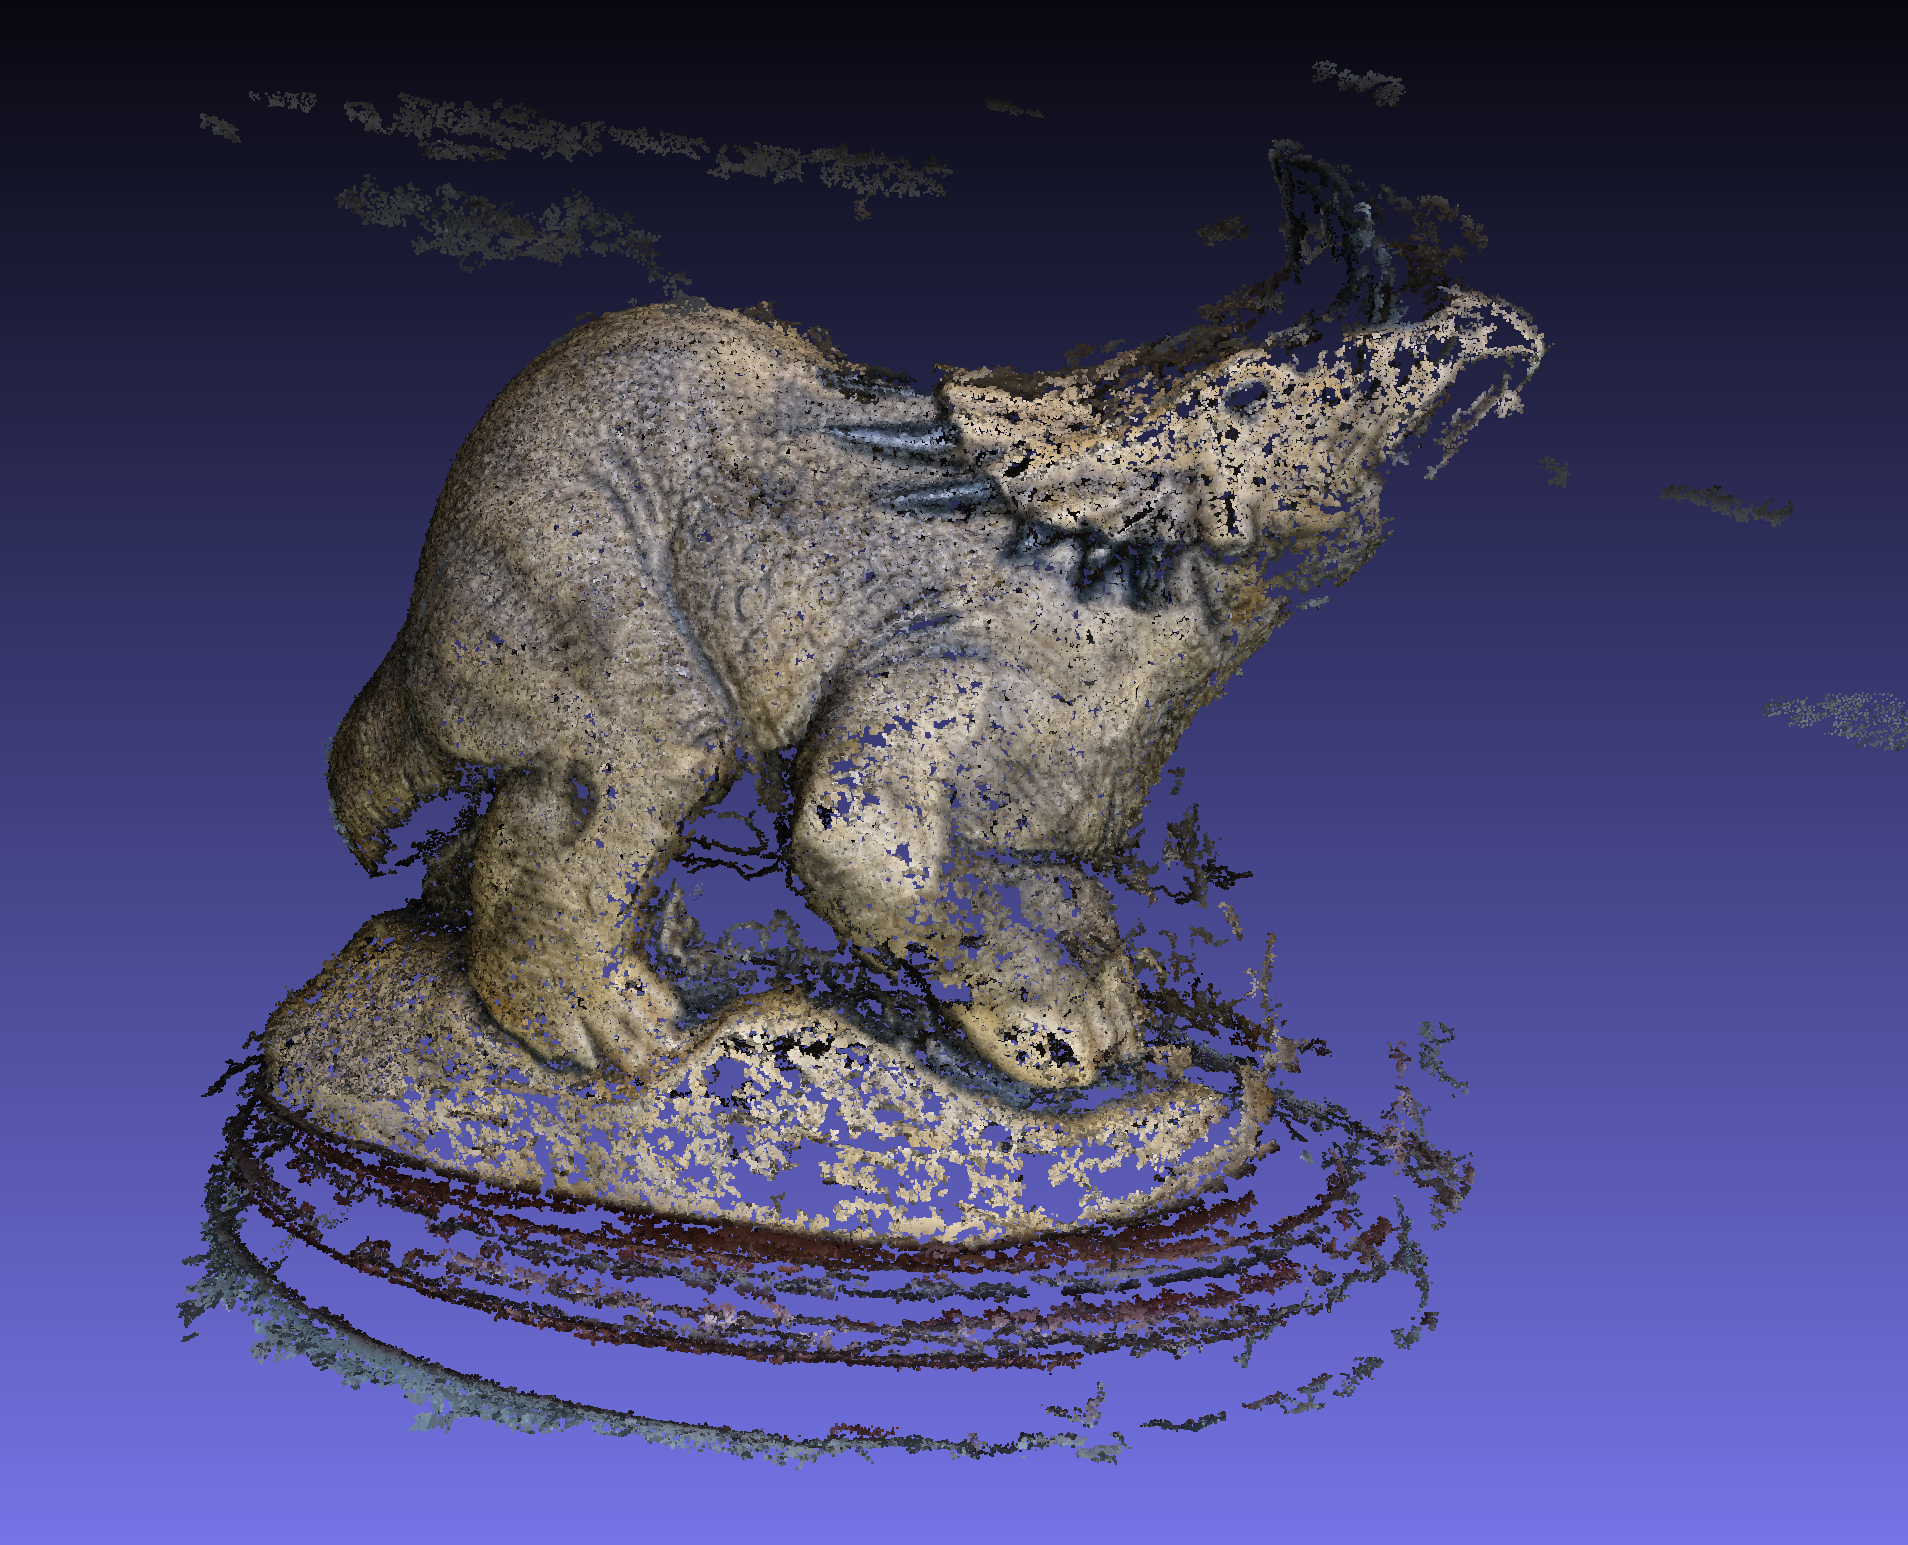
\includegraphics[width=\linewidth]{datas/state_of_the_art/visualsfm_result_dino.png}
        \caption{}
    \end{subfigure}

    \begin{subfigure}{0.45\textwidth}
        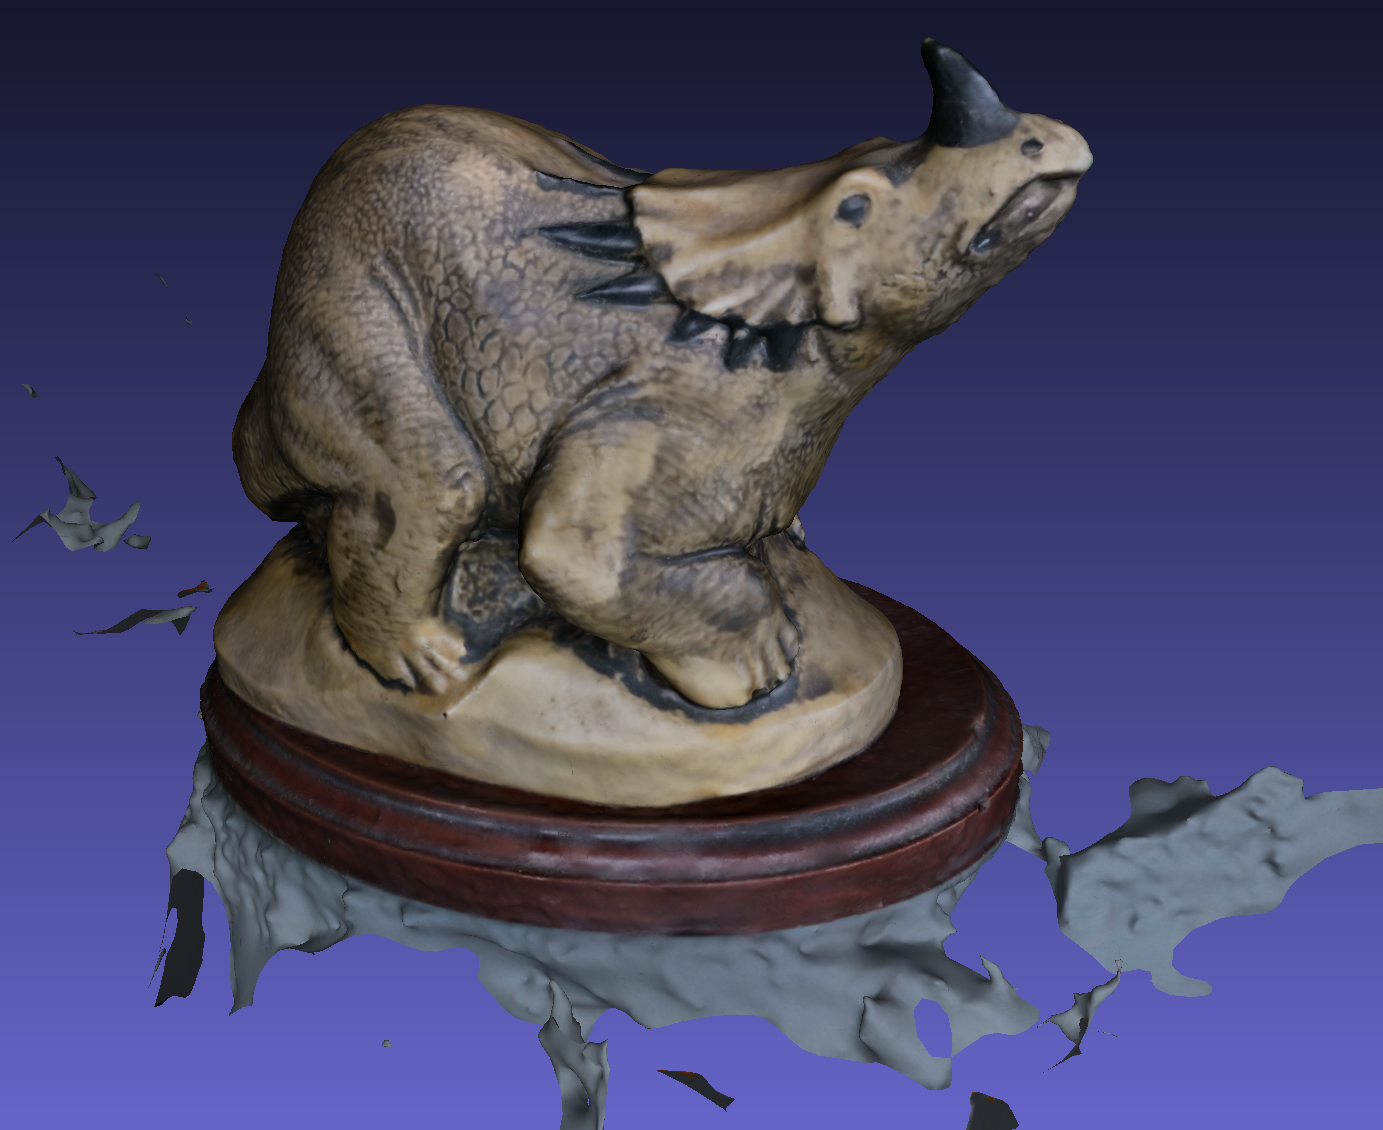
\includegraphics[width=\linewidth]{datas/state_of_the_art/openmvg_openmvs_result_dino.png}
        \caption{}
    \end{subfigure}
    \begin{subfigure}{0.45\textwidth}
        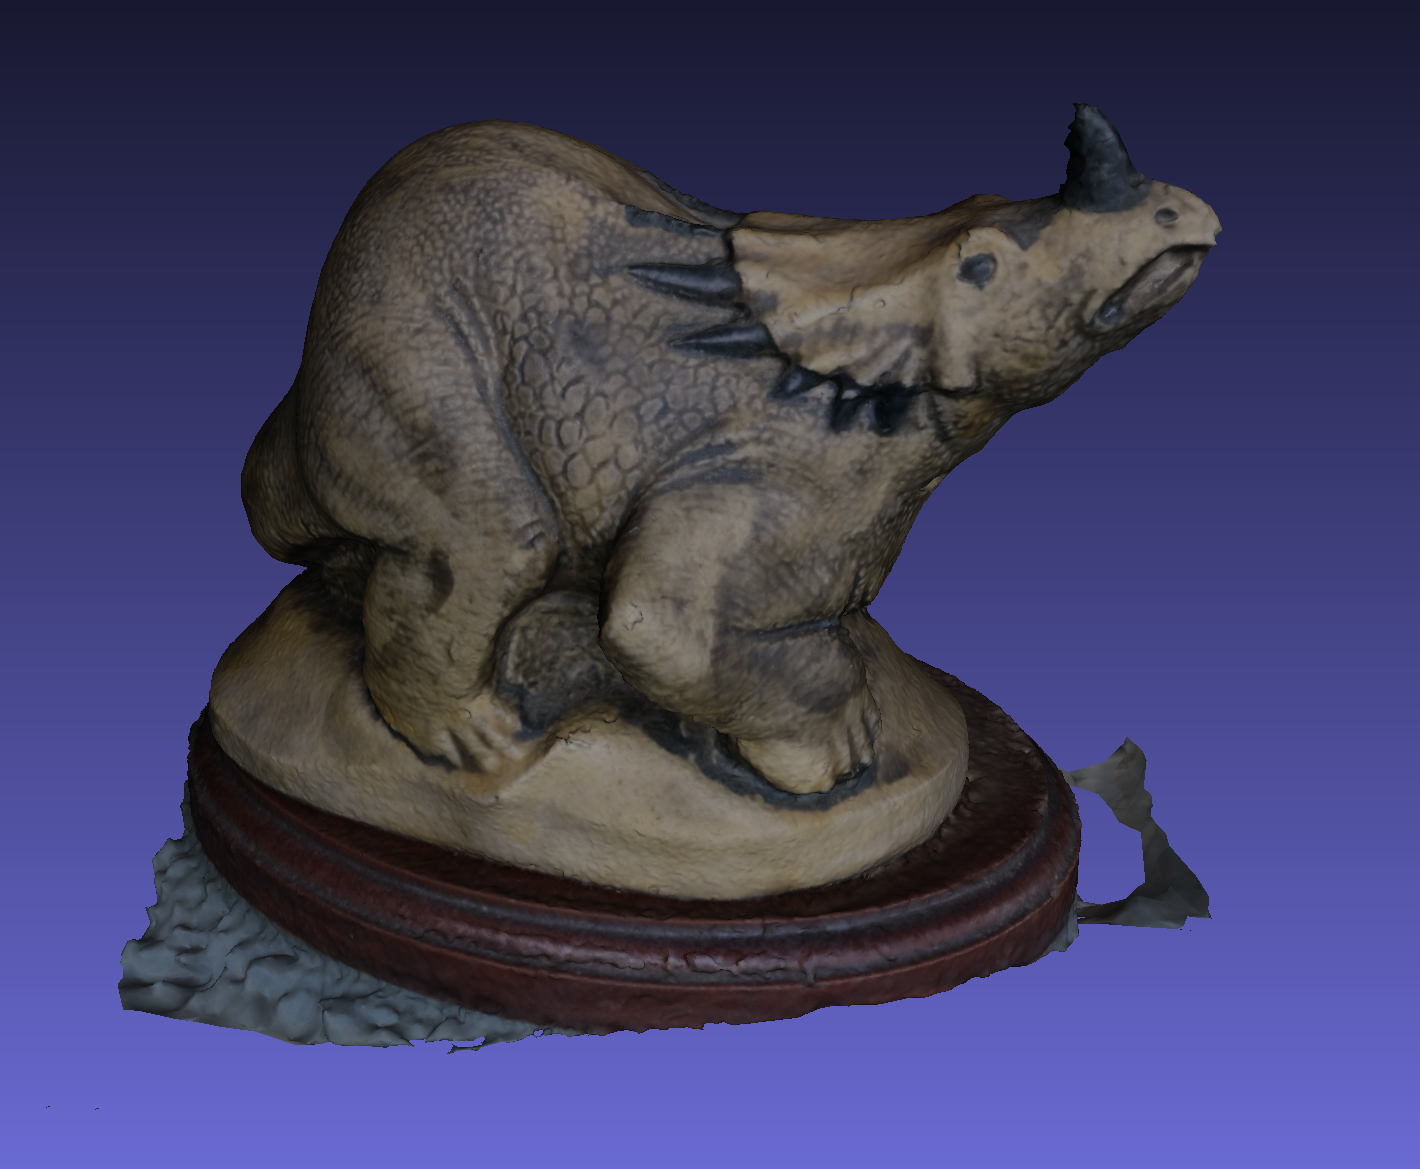
\includegraphics[width=\linewidth]{datas/state_of_the_art/meshroom_result_dino.png}
        \caption{}
    \end{subfigure}

    \begin{subfigure}{0.45\textwidth}
        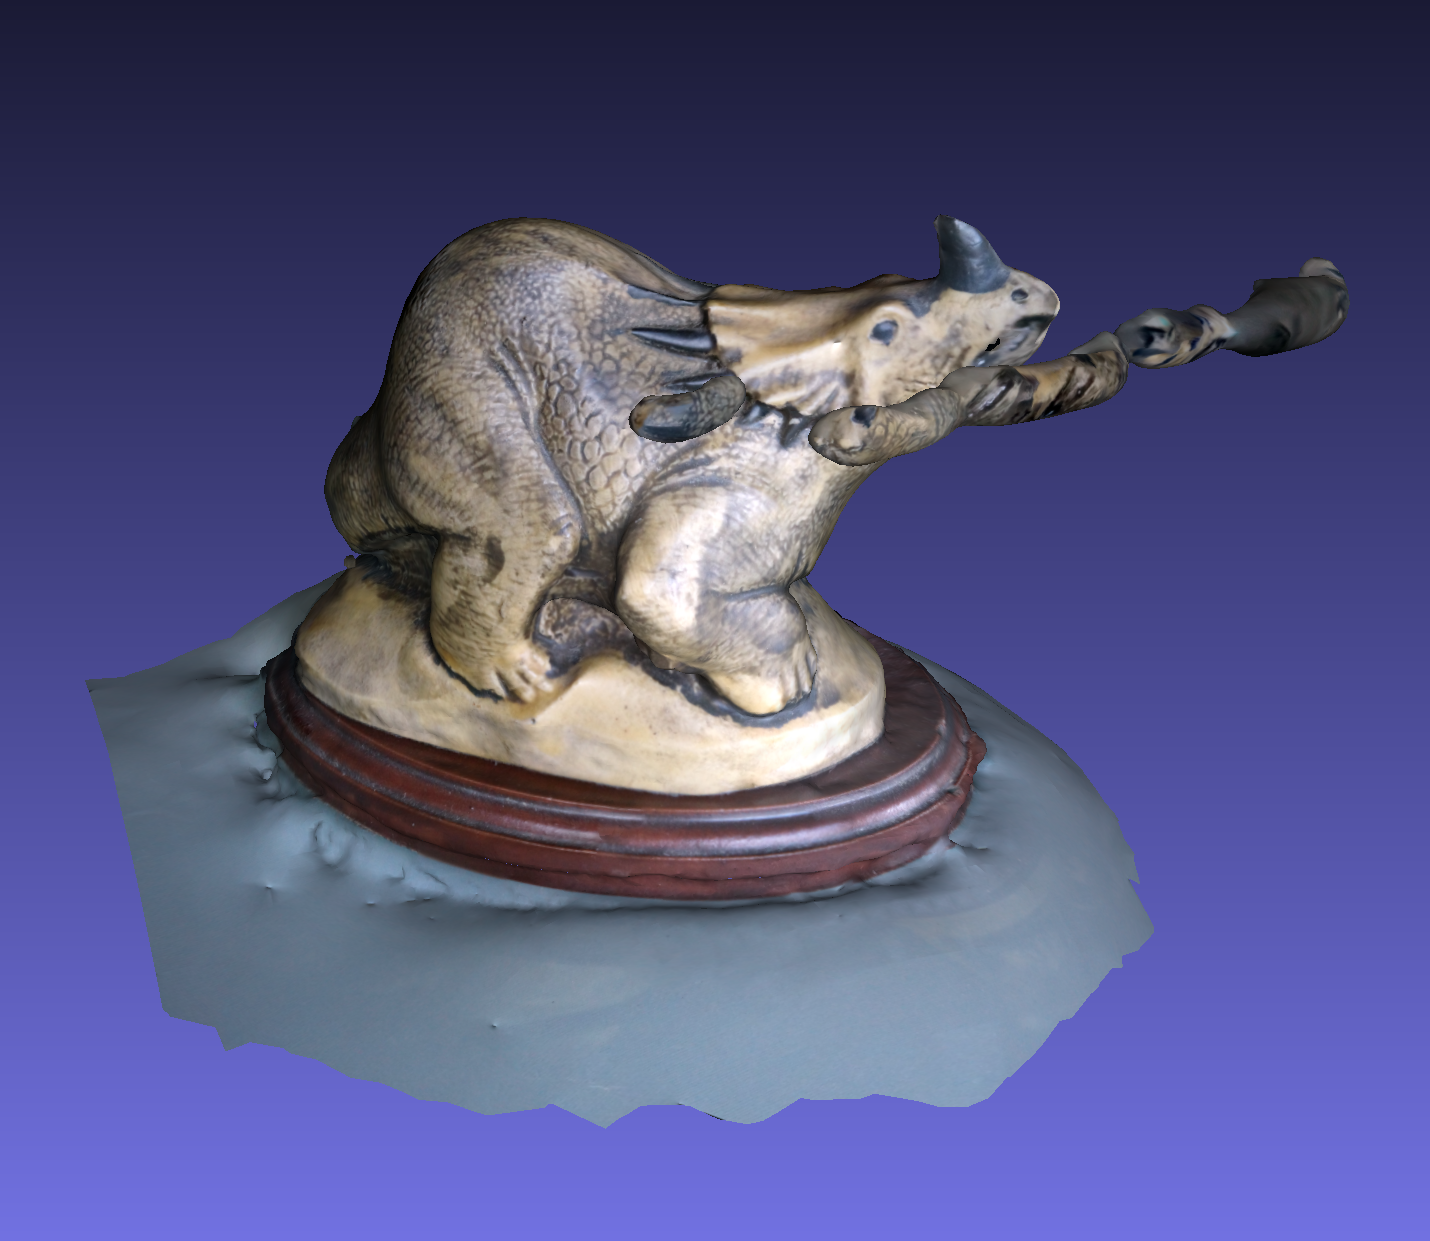
\includegraphics[width=\linewidth]{datas/state_of_the_art/regard3d_result_dino.png}
        \caption{}
    \end{subfigure}
    \begin{subfigure}{0.45\textwidth}
        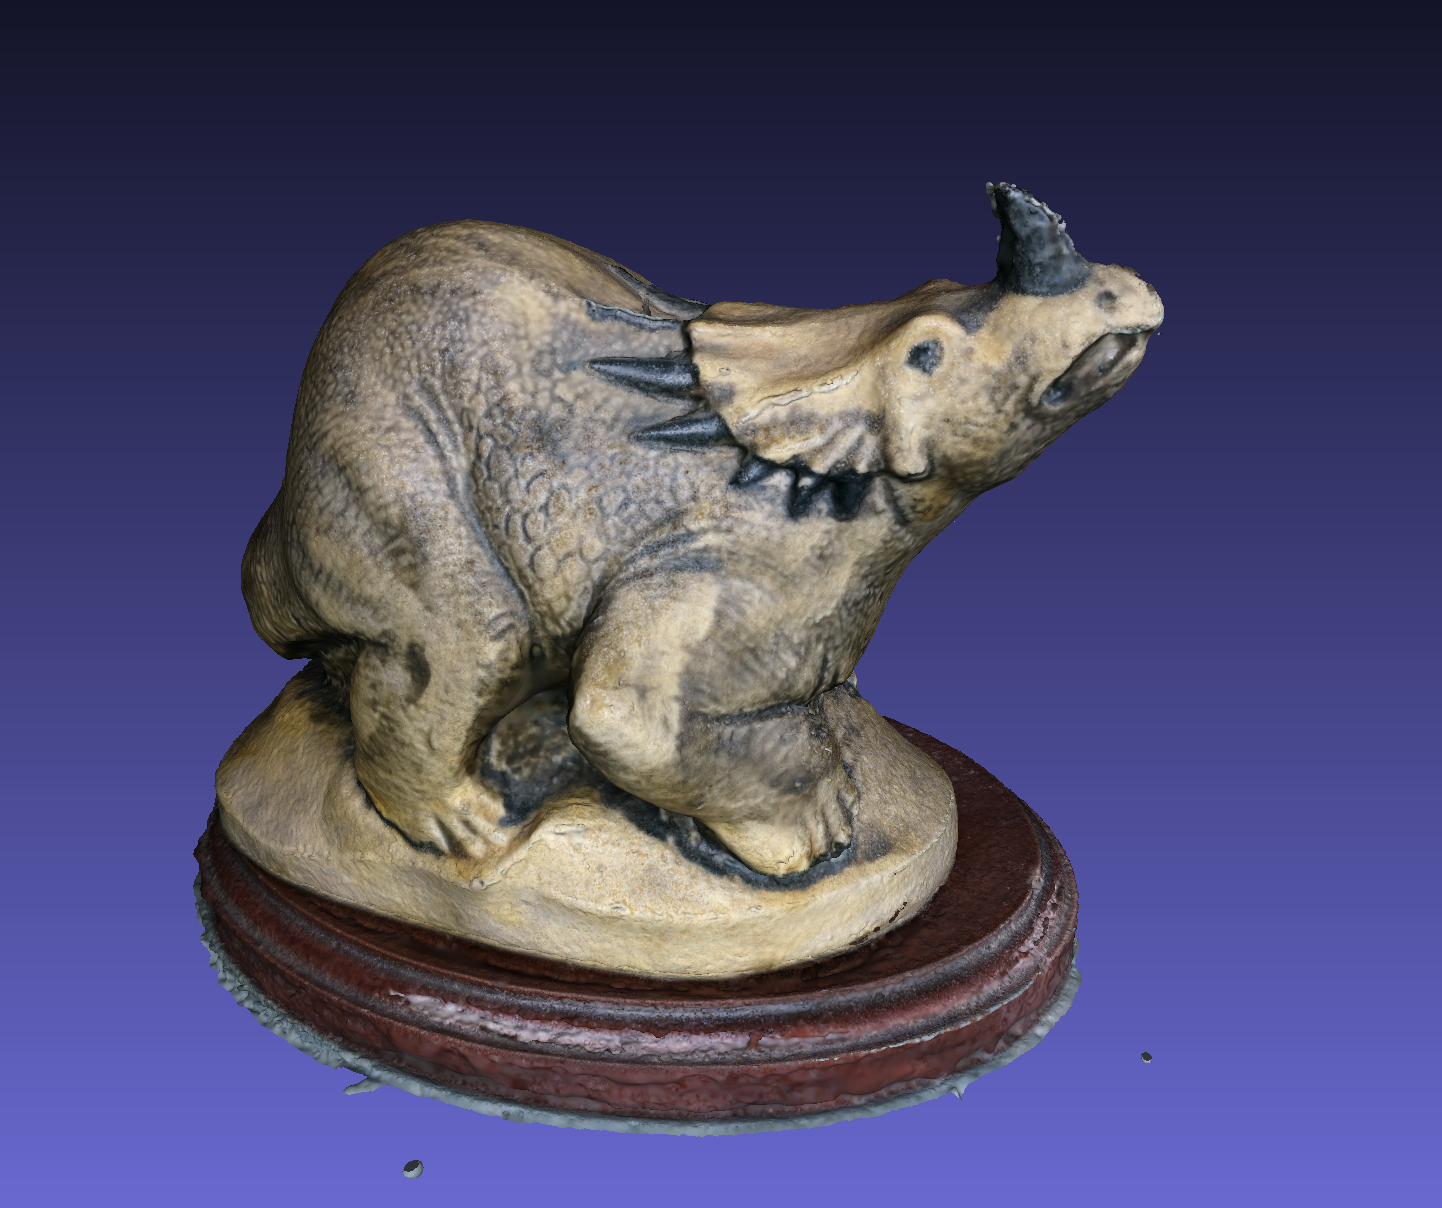
\includegraphics[width=\linewidth]{datas/state_of_the_art/colmap_result_dino.png}
        \caption{}
    \end{subfigure}

    \caption{Résultats de l'état de l'art avec le dataset Dinosaure : (a)OpenSFM, (b)VisualSFM, (c)OpenMVG+OpenMVS, (d)Alicevision Meshroom, (e)Regard3D, (f)Colmap}
    \label{fig:result_sota}
\end{figure}

\section{Choix final}

Explication du choix final

Transition vers la partie suivante